\section*{Goal}
The goal of this lab course was to get to know and learn how to set up Diode Lasers.
With the installed diode laser the fluorescence of Rubidium got analysed.
\section{Theory}
\label{sec:theory}
The theoretical background for Lasers and especially diode lasers needs to be understood to properly work with the setup.
In this chapter everything important for the lab course is explained.
\subsection{Lasers}
Laser (Light Amplification by Stimulated Emission of Radiation) is a form of Light emission which is frequently used in the industry and for research.
Light emitted from a Laser is coherent in time (all photons have the same phase) and space (the photons travel parallel in the same direction).
The Laser-light consists of photons with the same wavelength (monochromatic) and therefore the same energy, the photons also have the same linear polarization.
To produce the light a Laser consists out of three major parts: The active medium, the energy pump and the Resonator.

The active medium determines the wavelength of the photons because they are generated by the electrons relaxing over the band gap of the material.
To create laser light a population inversion has to be created with the different energy levels in the active medium.
If we assume three energy levels in the active medium with the first level $E_1$ having the lowest energy and the third level having the highest energy.
To create population inversion in the medium, the second level $E_2$ has to have more electrons than the first (lowest) level.
The relaxation from the third to the second level $E_2$ has to be a faster transition than the transition from the second energy level to the first level $E_1$ (ground state).
To provide enough electrons in the higher level a energy pump has to be used to excite electrons from the ground state $E_1$ to the third energy level.

To relax from the second level $E_2$ to the ground state $E_1$ the electrons can either spontaneously relax and emit the corresponding photon or can be stimulated by an incoming photon to relax and therefore emit a second photon with the same properties (Orientation, Frequency, Phase and Polarization).
This stimulated emission is the main source for the photons of the laser.
The simulated emission and the spontaneous emission are shown in figure \ref{fig:emission}.

When lasers travel onto rough materials they show a typical speckle pattern which is not seen for normal light \cite{speckle}.
The speckle pattern occurs, because different parts of the laser interfere with each other on the rough surface.
By hitting the surface, each illuminated point acts as a source for a new spherical wave and these waves can interfere and create the speckle pattern, if the surface is rough enough to create phase changes greater than $2\pi$.

\begin{figure}[ht]
    \center
    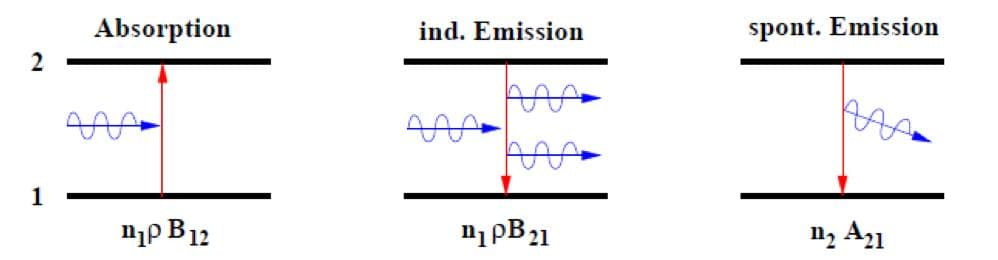
\includegraphics[width=0.8\textwidth]{bilder/emission.jpg}
    \caption{The absorption and emission processes in the active medium are shown for a two state system. \cite{anleitungHeNe}}
    \label{fig:emission}
\end{figure}

\subsection{Doped semiconductors}
\label{sec:doting}
To change the electrical properties of semiconductors the doting of the semiconductor is a widely used method.
Doting is the process of introducing atoms of another material with more (n-doped) or less (p-doped) valence electrons than the atoms of the semiconductor.
In p-doped semiconductors holes are the majority of the charge carriers and in n-doped semiconductors electrons are the majority of the charge carriers.
By doting the semiconductor the Fermi-energy inside the material is changed \ref{fig:doting} and another energy level is introduced.

\begin{figure}
    \centering
    \begin{subfigure}{0.49\textwidth}
        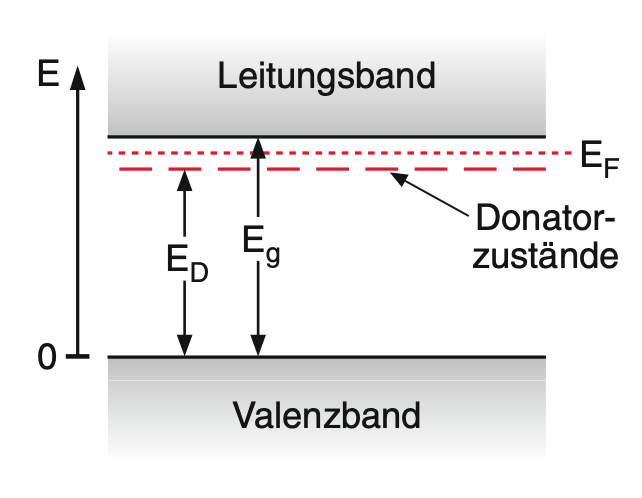
\includegraphics[width = \textwidth]{bilder/n_Donatorschema_demtroeder.png}
        \caption{n-doped}
    \end{subfigure}
    \hfill
    \begin{subfigure}{0.49\textwidth}
        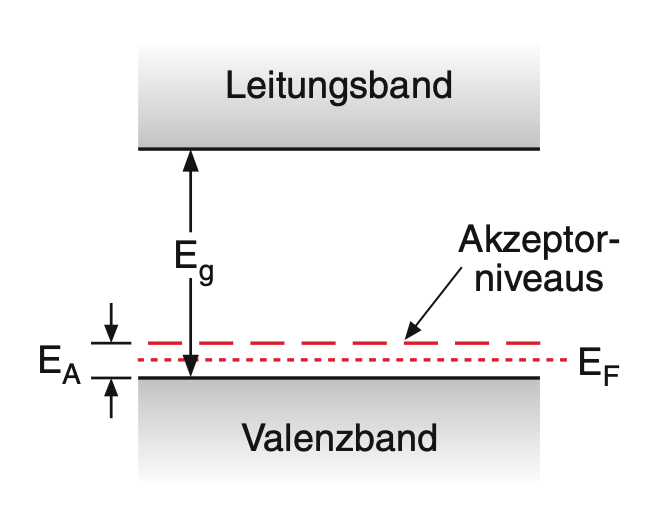
\includegraphics[width = \textwidth]{bilder/p_Donatorschema_demtroeder.png}
        \caption{p-doped}
    \end{subfigure}
    \caption{The Band structures with the fermi energy and the donor and acceptor states sre shown for p- and n-doped materials \cite{demtroeder}}
    \label{fig:doting}
\end{figure}

\subsection{Diode Laser}
In this experiment a pn-junction diode is used.
A pn-junction diode is a part of a electrical circuit.
The diode has a positive and negative direction and only allows the current to pass the diode in the positive direction.
A pn-junction consists of two semiconductors (one p doped and another n doped \ref{sec:doting}) which are combined to build the junction at the border.
By applying a current to the diode, the holes and the electrons meet in junction region and recombine.
During the recombination the laser photons get emitted and due to the internal reflection stimulated emission occurs in the medium.
Because the Diode produces a laser which is strongly diverging and has a big frequency width  a external optical setup is used (seen in figure \ref{fig:assembly2} and more deeply explained in section \ref{sec:grating}).
With a lens the diverging laser is transformed in a parallel light and then pointed onto a grid surface.
\cite{laser_diode}

\subsection{Gain Curves}
\label{sec:gain}
\begin{figure}
    \center
    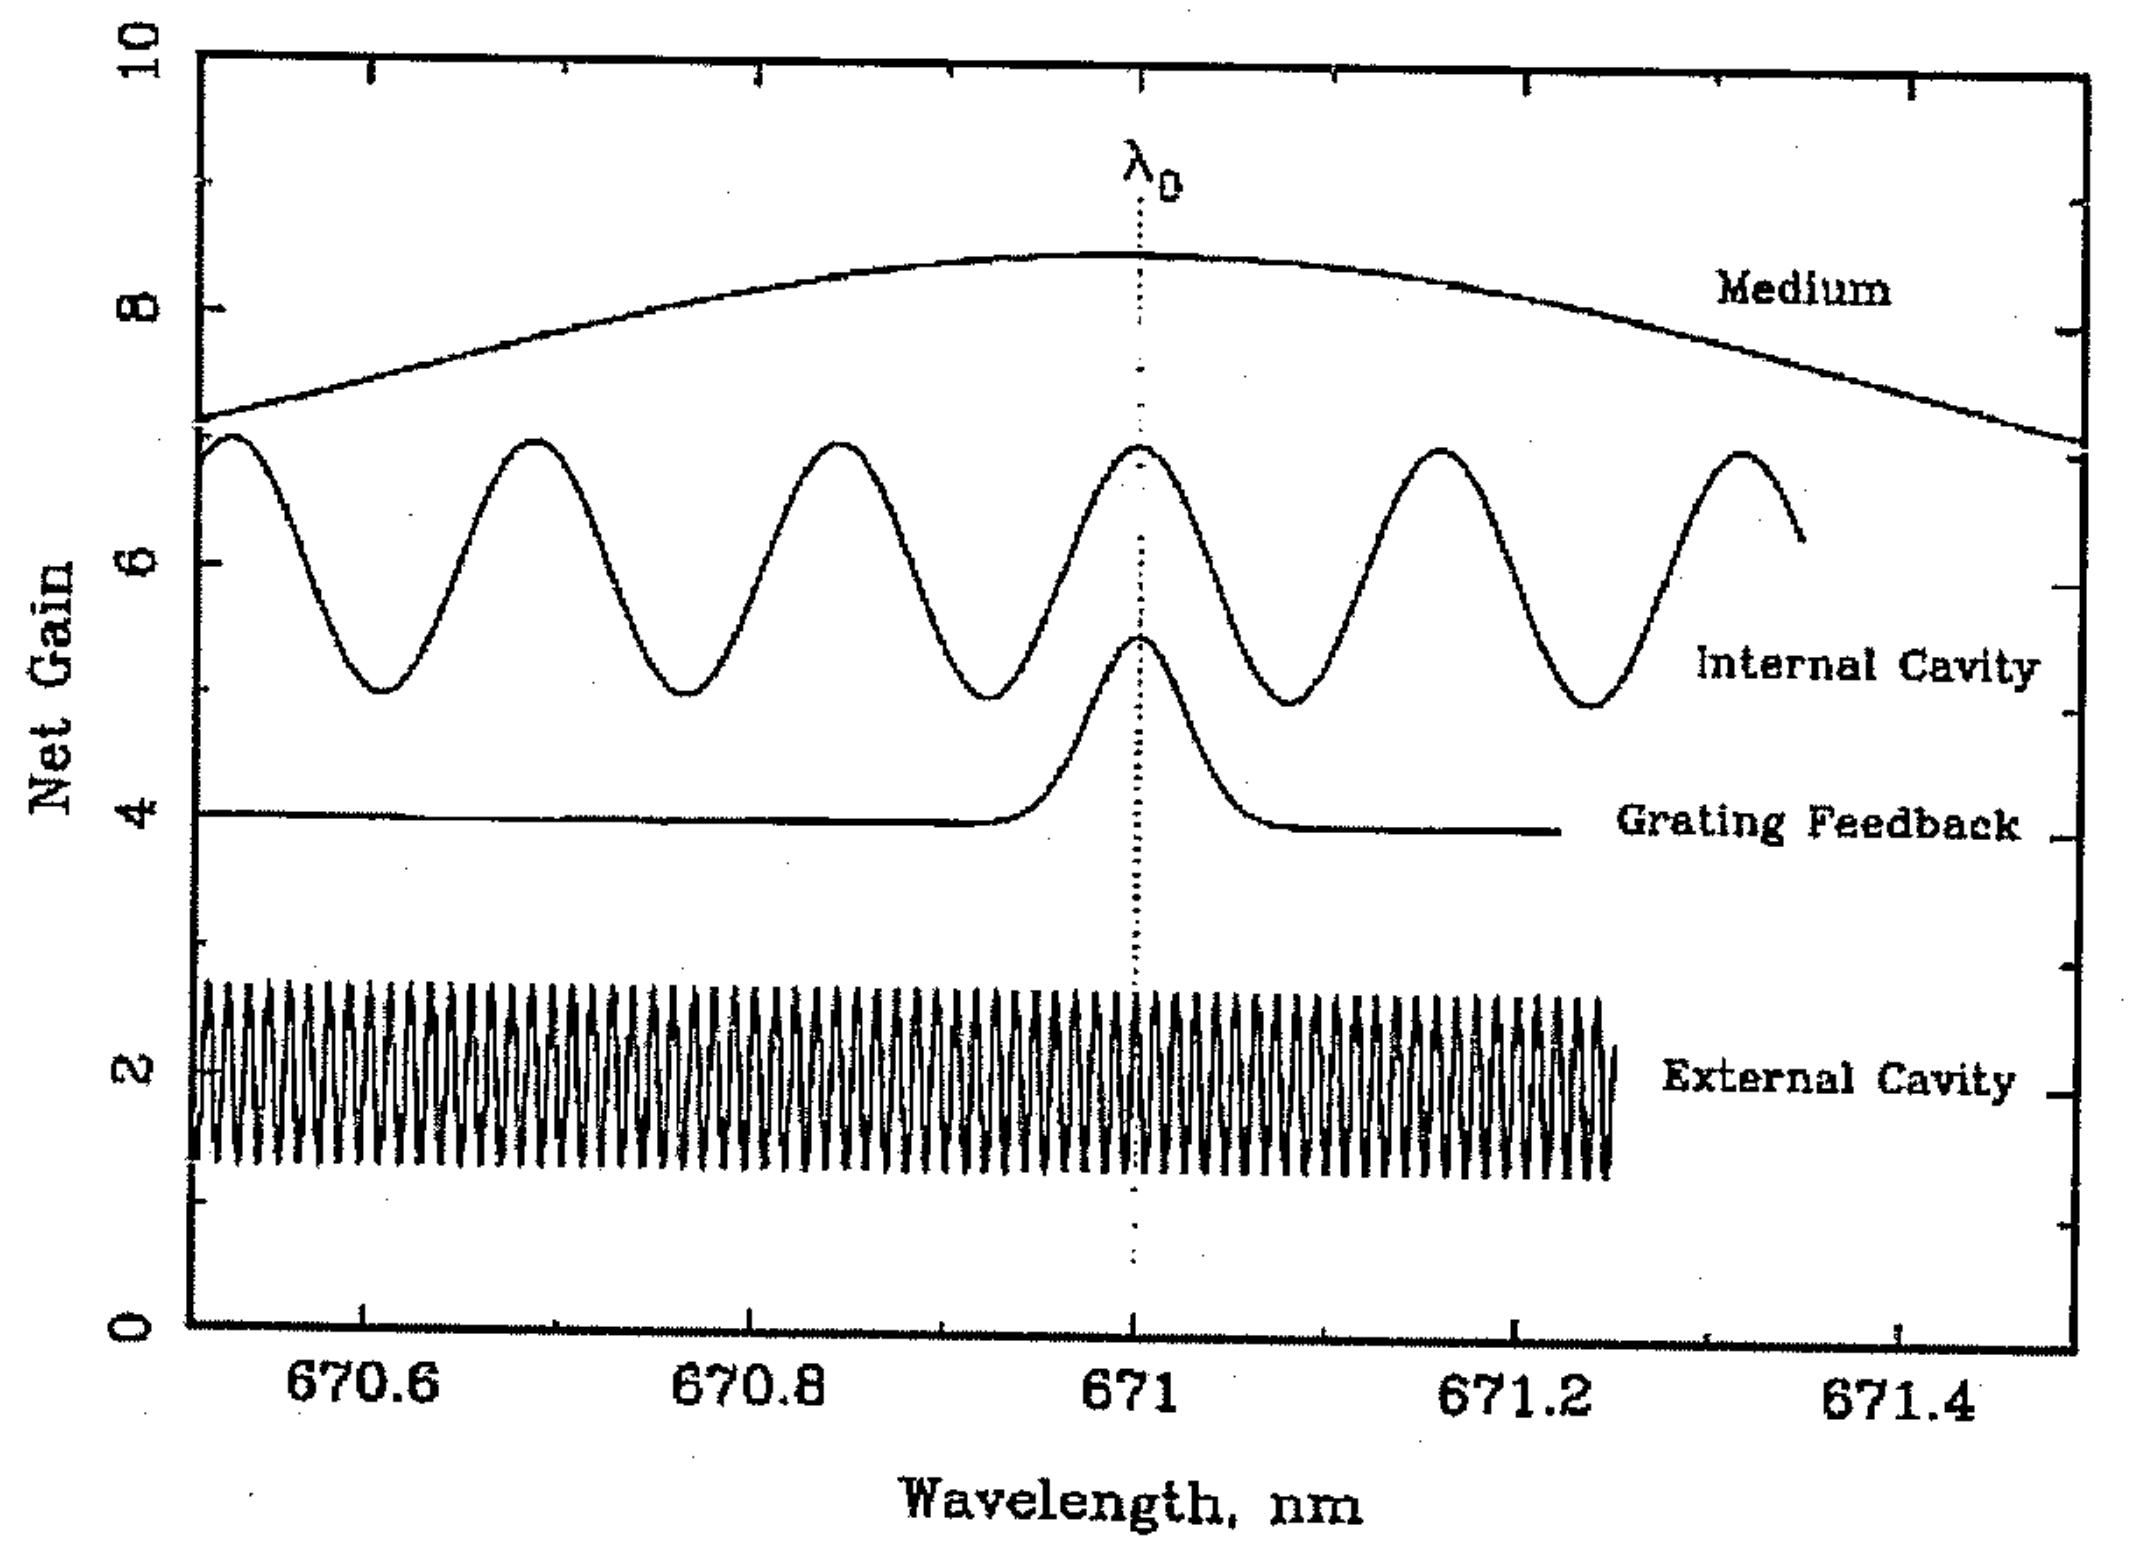
\includegraphics[width=0.8\textwidth]{bilder/Gain_curve.png}
    \caption{The different parts of the Gain Curves of the Diode laser are shown separately. By adjusting the different parts the wanted frequency can be reached \cite{anleitung}}
    \label{fig:gain}
\end{figure}
\subsubsection{Medium Gain}
The medium band gap dictates the energy and therefore the frequency/wavelength of the photons.
The medium gain curve is very broad for the temperature region in the experiment (which is chosen for the \SI{780}{\nano \metre} of the rubidium resonance).
\subsubsection{Internal Cavity}
The internal cavity is the standing wave due to the reflection inside the medium.
This kind of laser is called 'Fabry-Perot-Laser-Diode' but for a material like GaAs an additional set of mirrors is not necessary because on the border of the medium to air a reflection of \num{0.32} is reached.
Due to the standing wave the frequency of the laser is dependent on the length of the active medium. 
\subsubsection{Grating Feedback and external cavity}
\label{sec:grating}
To determine the frequency emitted by the laser instead of the internal cavity, also a external resonator is used.
To get a frequency selection an optical grating is placed in front of the laser with a lens between the diode and the grating.
The grating is assembled in a way to reflect the first order of reflection, which travels back into the diode.
The frequency of the laser light is then dependent on the angle of the grating and can be varied by turning the Grating.
This assembly of a laser feedback is called a Littrow Laser(Kap 10.5.3 \cite{eichler_laser}).
\subsection{Rubidium}
Rubidium has two stable isotopes, $^{85}Rb$ and $^{87}Rb$.
In figure \ref{fig:rubidium} the energy states of the isotopes and the relaxation paths are shown.
The relaxations (denoted by a and b) can be associated to the different signals of the transmission spectrum of rubidium.
\cite{rubidium}
\begin{figure}
    \center
    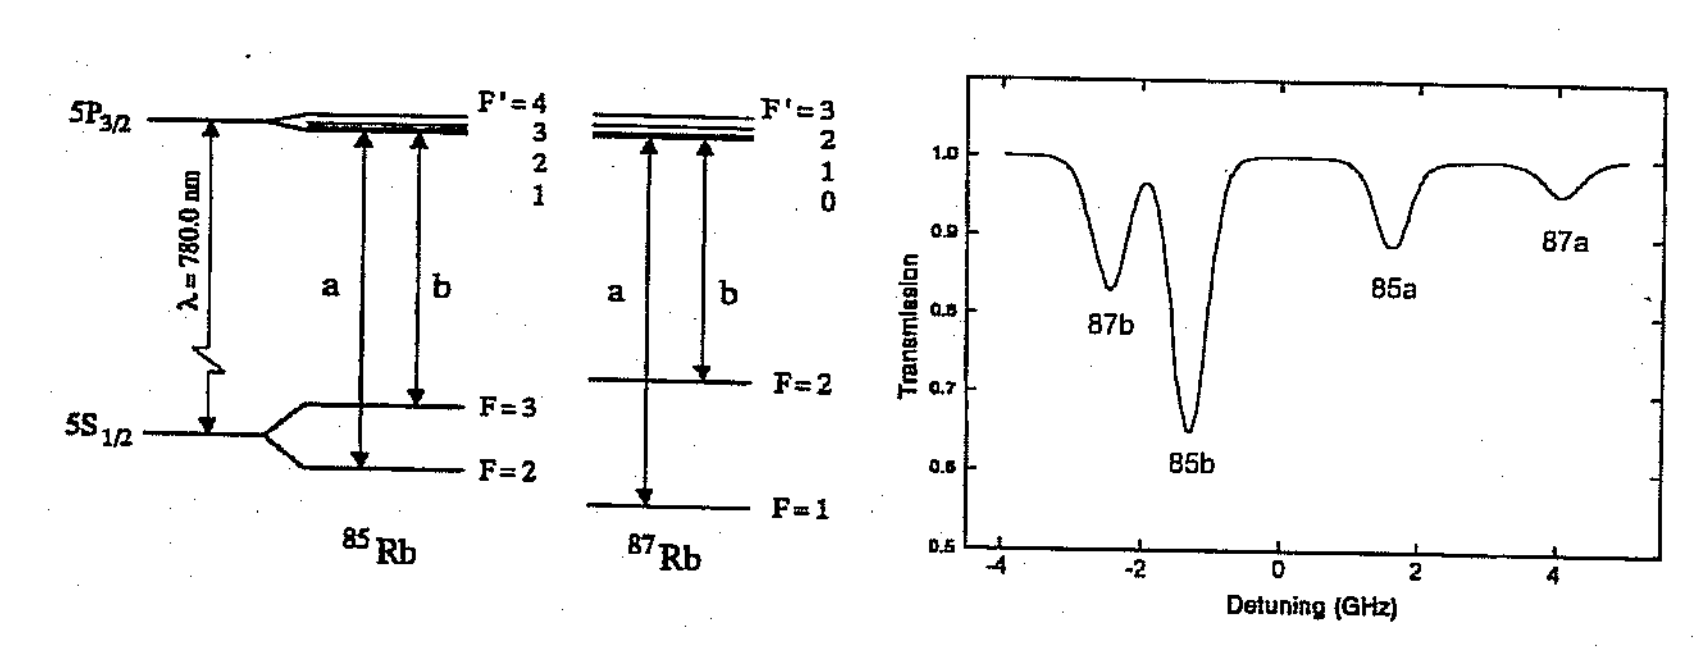
\includegraphics[width=0.8\textwidth]{bilder/Rubidium_Energy.png}
    \caption{On the left side the energy levels of $^{85}Rb$ and $^{87}Rb$ are shown. On the right side the corresponding transmission spectrum of rubidium at wavelength near \SI{780}{\nano \metre} is shown. \cite{anleitung}}
    \label{fig:rubidium}
\end{figure}